\clearpage
\paragraph{Soggetto 2}~

\vspace{1cm}

\noindent In questo paragrafo, vengono presentate le misurazioni effettuate su un soggetto di sesso femminile, di età 41 anni e carnagione chiara. Il soggetto si trovava in condizioni di riposo.

\vspace{0.5cm}

\noindent Di seguito sono riportate le acquisizioni effettuate utilizzando il sensore \textbf{MAX86916} su una finestra temporale di 10 secondi.

\subparagraph{Polpastrello indice sinistro}
Dalle acquisizioni riportate in figura \ref{fig:soggetto2_MAX86916_polpastrello}, effettuate sul polpastrello dell'indice della mano sinistra, si può notare come il segnale ottenuto sia di ottima qualità per tutte e quattro le lunghezze d'onda impiegate, confermando i risultati ottenuti con il soggetto 1, e anche le considerazioni fatte a livello teorico nel capitolo \ref{cap:sitimisura}. Infatti, dalle immagini riportate si possono distinguere chiaramente sia i picchi sistolici, sia diastolici e le tacche dicrotiche. Anche qui si possono individuare 10 picchi del segnale, stimando una frequenza cardiaca di 60 battiti al minuto.\todo{direi che il segnale con ampiezza maggiore è decisamente il verde, inserire la frase}
\begin{figure}[h]
	\centering
	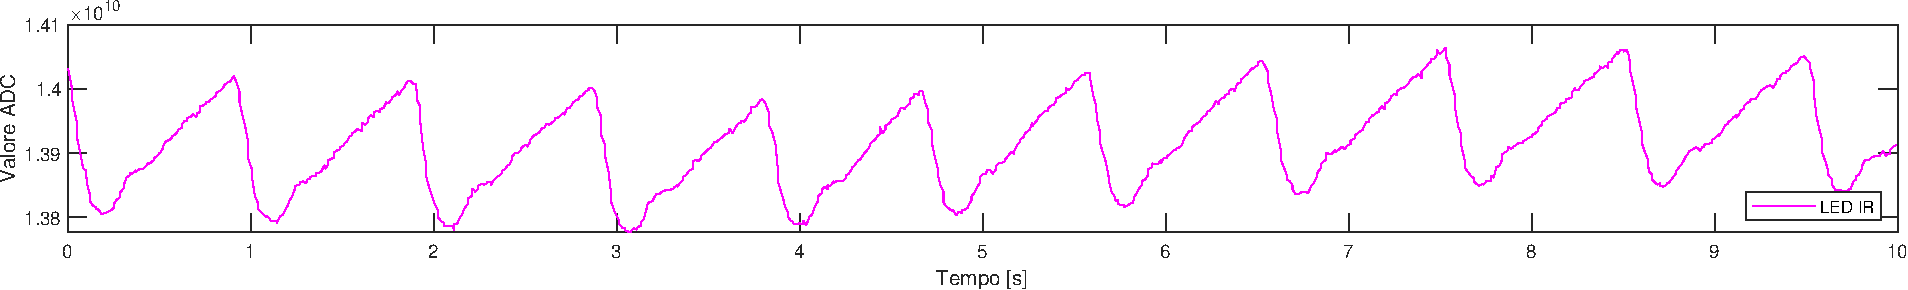
\includegraphics[width=1\linewidth]{ImageFiles/Misure Preliminari/Soggetto 2/max86916/polpastrello_ired}
	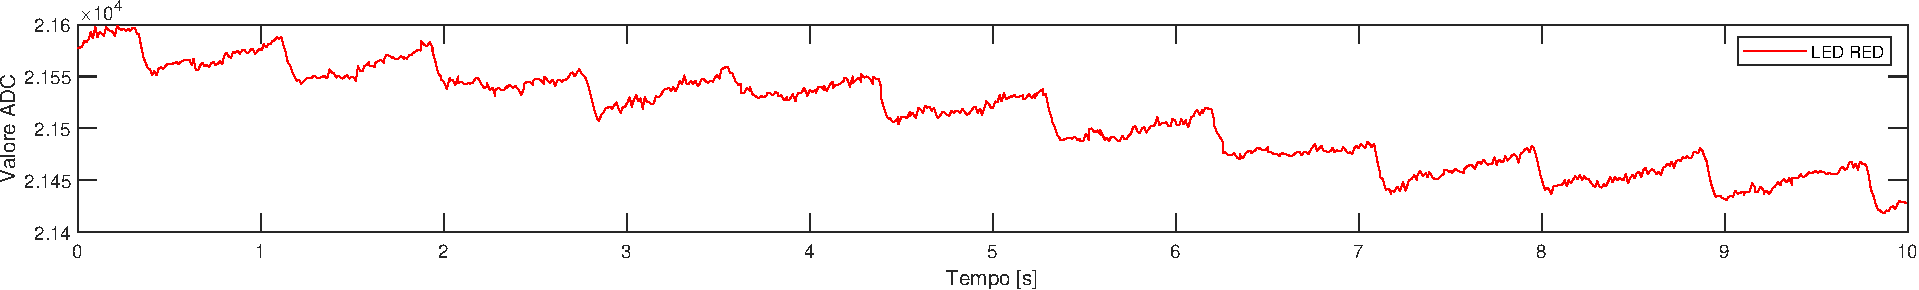
\includegraphics[width=1\linewidth]{ImageFiles/Misure Preliminari/Soggetto 2/max86916/polpastrello_red}
	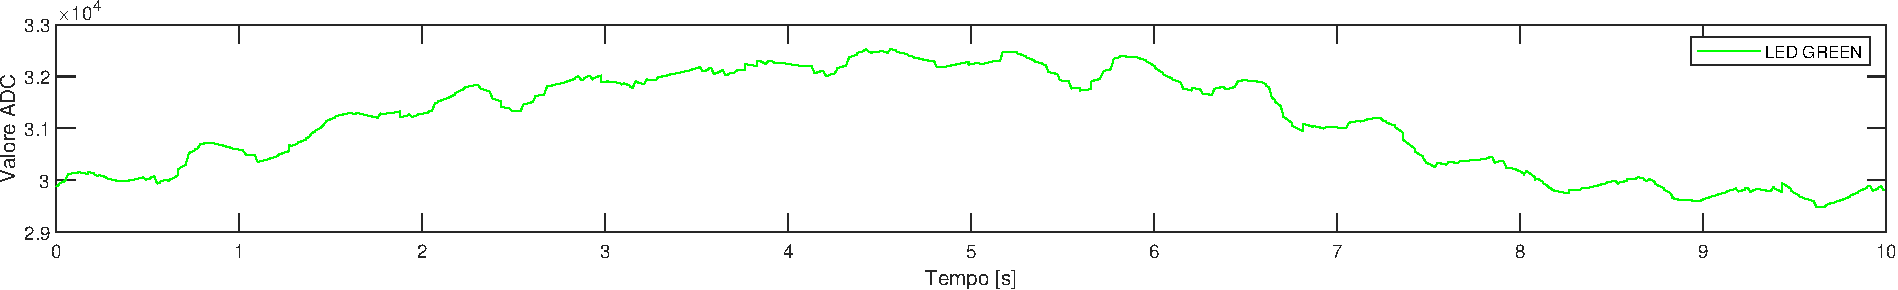
\includegraphics[width=1\linewidth]{ImageFiles/Misure Preliminari/Soggetto 2/max86916/polpastrello_green}
	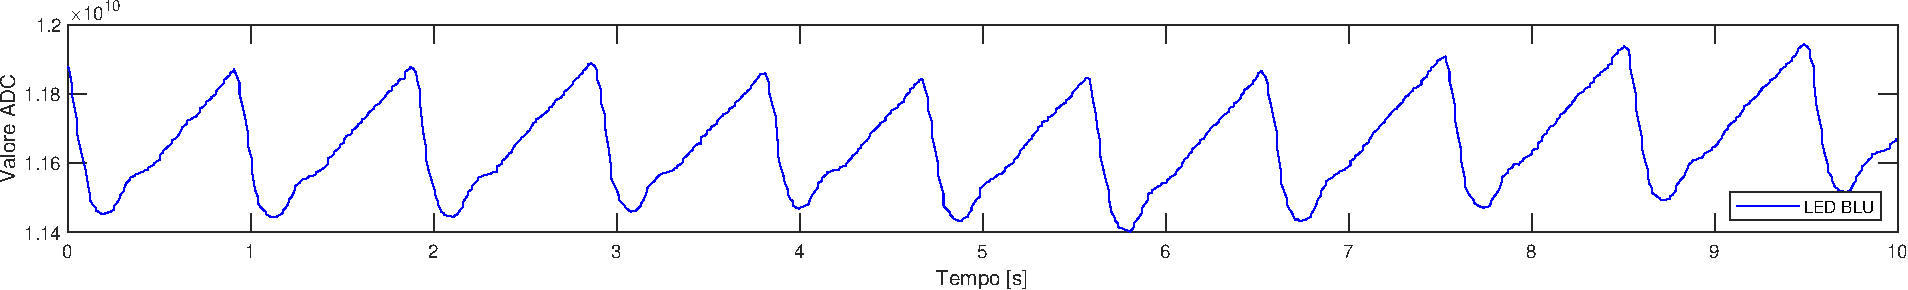
\includegraphics[width=1\linewidth]{ImageFiles/Misure Preliminari/Soggetto 2/max86916/polpastrello_blu}
	\caption{MAX86916: segnali PPG acquisiti sul polpastrello del dito indice sinistro.}
	\label{fig:soggetto2_MAX86916_polpastrello}
\end{figure}

\clearpage

\paragraph{Lobo orecchio sinistro}
Le acquisizioni ottenute sul lobo dell'orecchio sinistro presentano un segnale di qualità leggermente inferiore rispetto al sito precedente. Ciò è dovuto principalmente alla difficoltà della misura in questo sito. Tuttavia, la morfologia del segnale è evidente. Infatti, in figura \ref{fig:soggetto2_MAX86916_lobo}, si possono ancora apprezzare i picchi sistolici e diastolici su tutte le lunghezze d'onda impiegate. I picchi individuati sono 10, stimando una frequenza cardiaca di 60 battiti al minuto, coerente con il risultato ottenuto con la misura sul polpastrello.
\todo{il maggiore mi sembra il verde}
\begin{figure}[h]
	\centering
	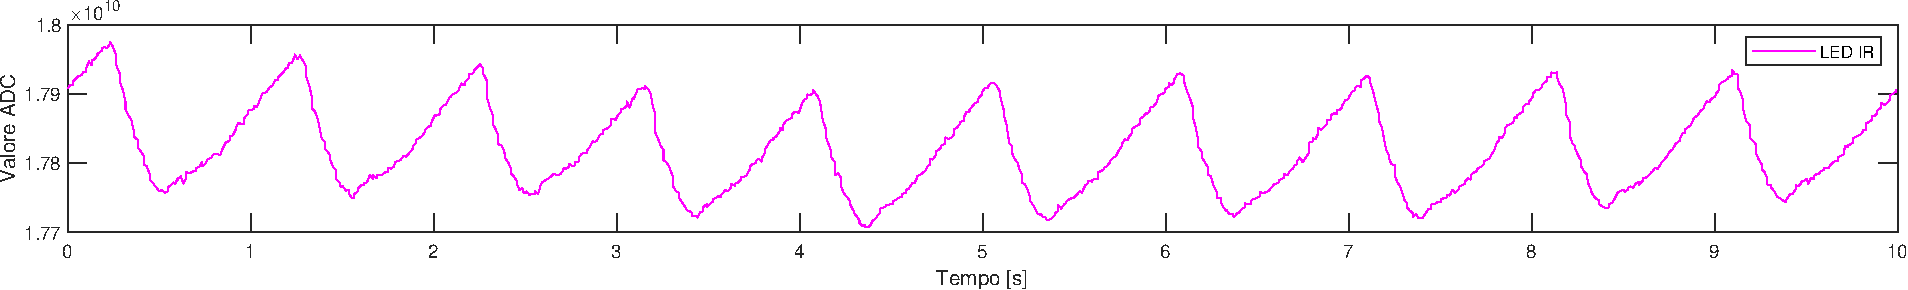
\includegraphics[width=1\linewidth]{ImageFiles/Misure Preliminari/Soggetto 2/max86916/lobo_ired}
	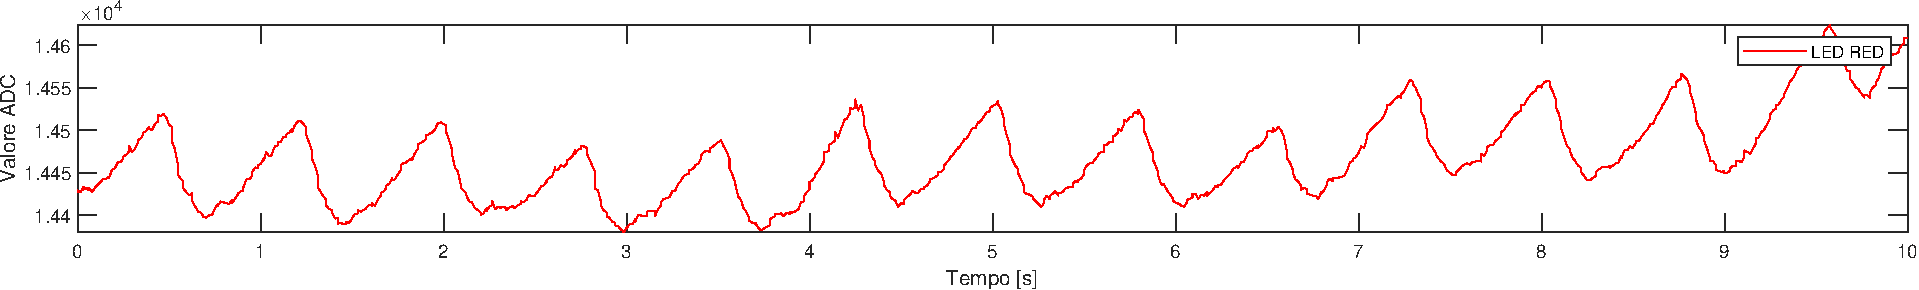
\includegraphics[width=1\linewidth]{ImageFiles/Misure Preliminari/Soggetto 2/max86916/lobo_red}
	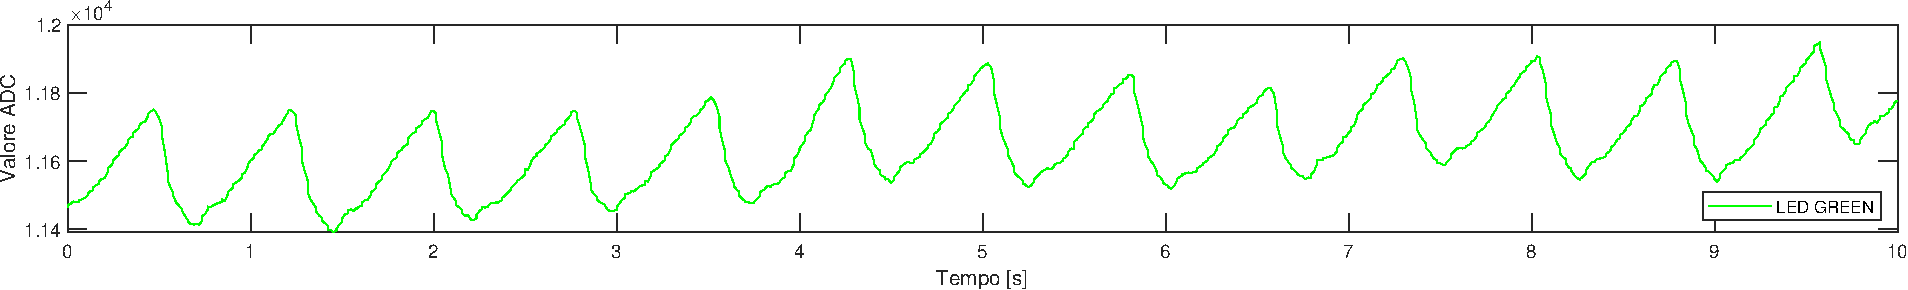
\includegraphics[width=1\linewidth]{ImageFiles/Misure Preliminari/Soggetto 2/max86916/lobo_green}
	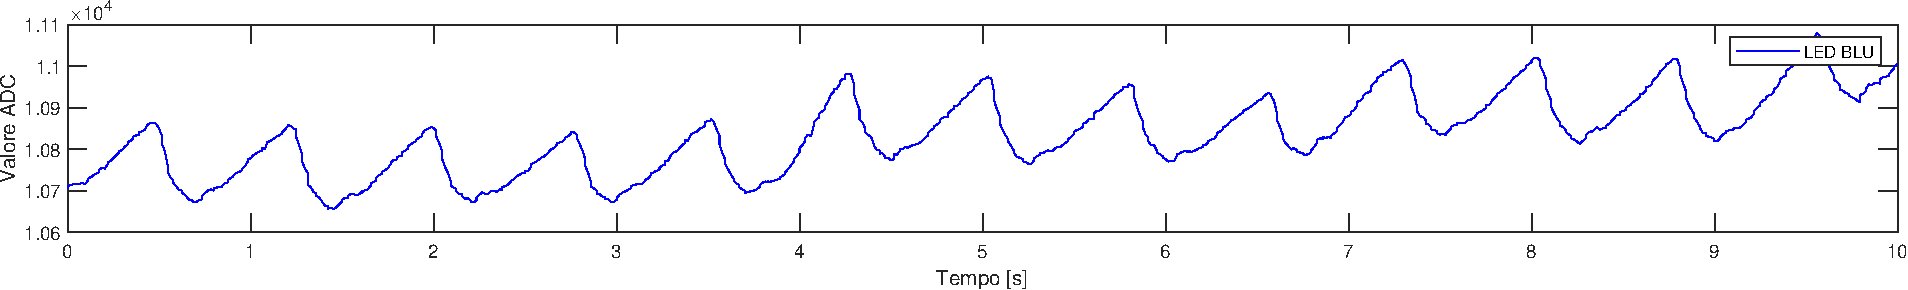
\includegraphics[width=1\linewidth]{ImageFiles/Misure Preliminari/Soggetto 2/max86916/lobo_blu}
	\caption{MAX86916: segnali PPG acquisiti sul lobo dell'orecchio destro.}
	\label{fig:soggetto2_MAX86916_lobo}
\end{figure}

\clearpage

\subparagraph{Polso antero-interno sinistro}

Le misure effettuate sulla zona del polso antero-interno sono più soggette a disturbi, principalmente dovute sempre a movimenti di natura involontaria. Come si può vedere in figura \ref{fig:soggetto2_MAX86916_polso}, questi disturbi sono più visibili per la luce rossa e infrarossa, mentre per la luce blu e verde il segnale si dimostra ancora pulito e chiaro. Nonostante ciò la qualità si può reputare buona, infatti sono ancora individuabili i picchi di interesse. La frequenza cardiaca stimata da questa acquisizione è di 63 battiti al minuto.\todo{maggiore verde vero? inserire frase}
\begin{figure}[h]
	\centering
	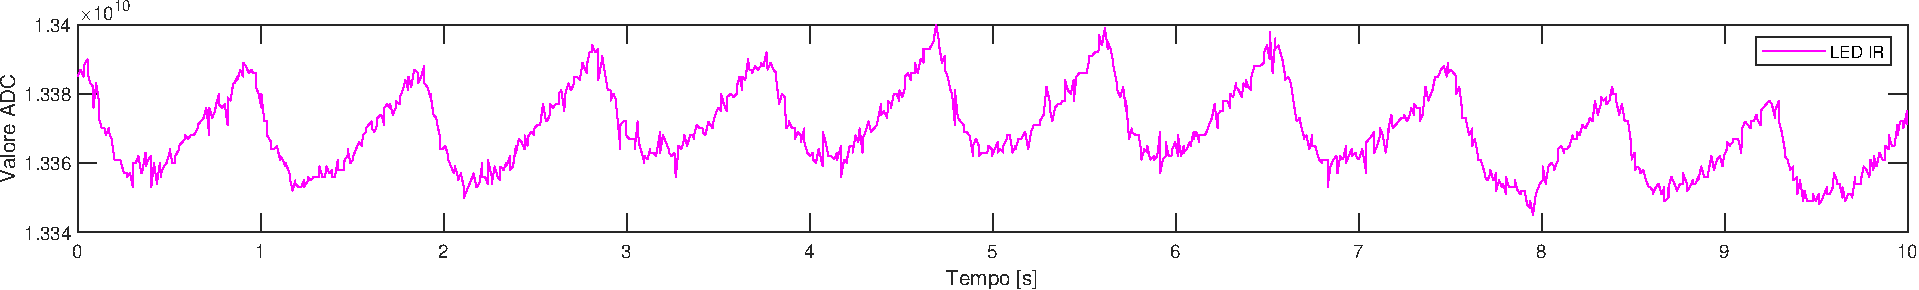
\includegraphics[width=1\linewidth]{ImageFiles/Misure Preliminari/Soggetto 2/max86916/polso_inferiore_ired}
	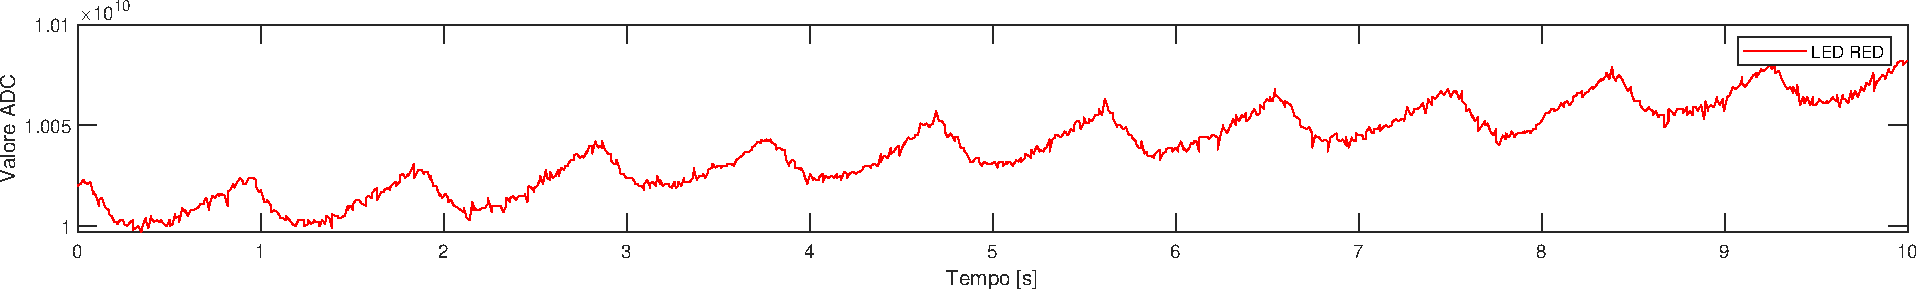
\includegraphics[width=1\linewidth]{ImageFiles/Misure Preliminari/Soggetto 2/max86916/polso_inferiore_red}
	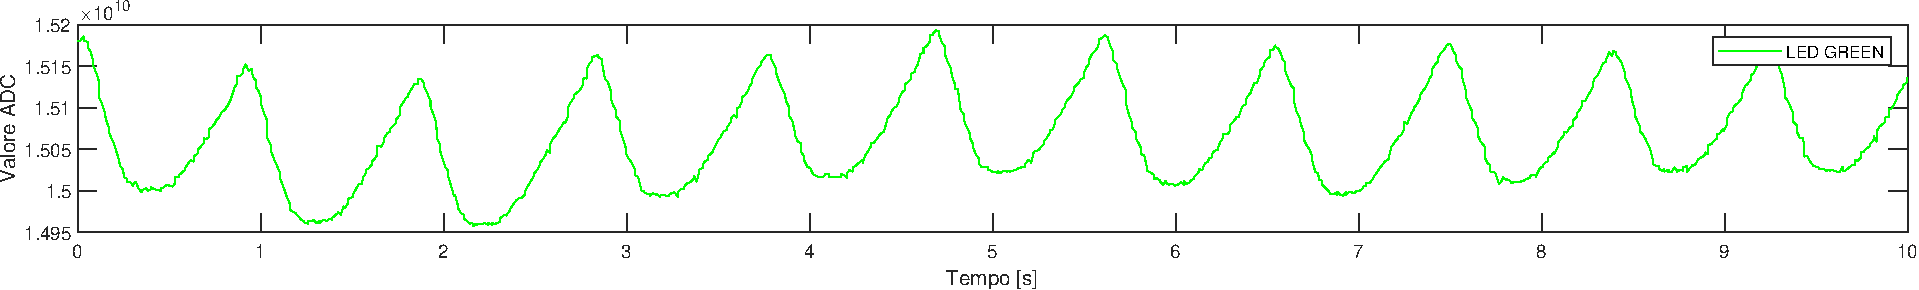
\includegraphics[width=1\linewidth]{ImageFiles/Misure Preliminari/Soggetto 2/max86916/polso_inferiore_green}
	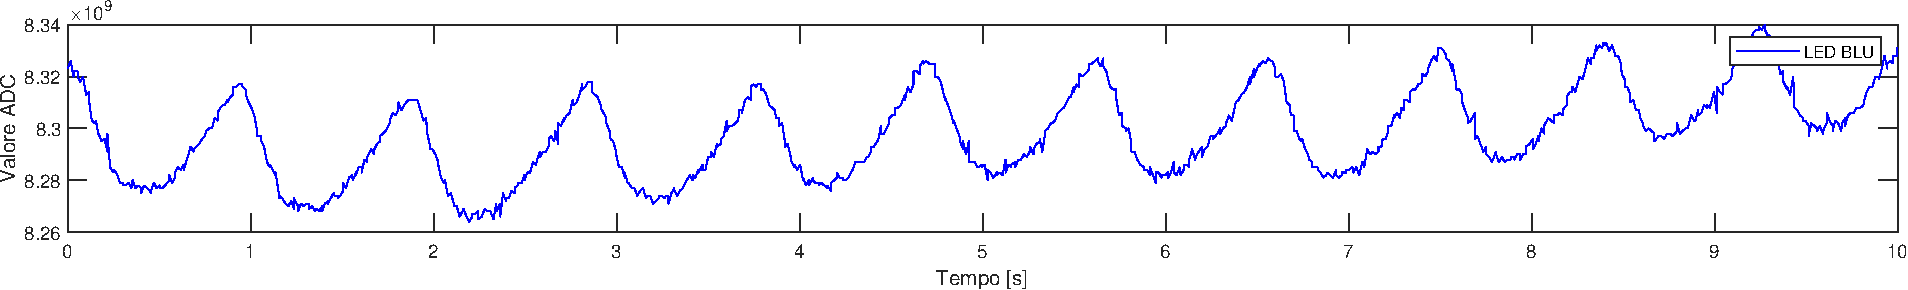
\includegraphics[width=1\linewidth]{ImageFiles/Misure Preliminari/Soggetto 2/max86916/polso_inferiore_blu}
	\caption{MAX86916: segnali PPG acquisiti sul polso destro.}
	\label{fig:soggetto2_MAX86916_polso}
\end{figure}

\clearpage

\subparagraph{Fronte}
Infine, in figura \ref{fig:soggetto2_MAX86916_lobo}, vengono riportati i risultati delle acquisizioni effettuate sulla fronte. I segnali ottenuti presentano una buona qualità. Osservando la componente AC dei segnali, il verde presenta un'ampiezza maggiore. Anche in questo caso si vede che la luce blu permette di identificare correttamente i picchi sistolici. Le misurazioni risultano essere meno rumorose rispetto a quelle acquisite sul polso. La frequenza cardiaca stimata è di 60 battiti al minuto, confermando i precedenti risultati.

\begin{figure}[h]
	\centering
	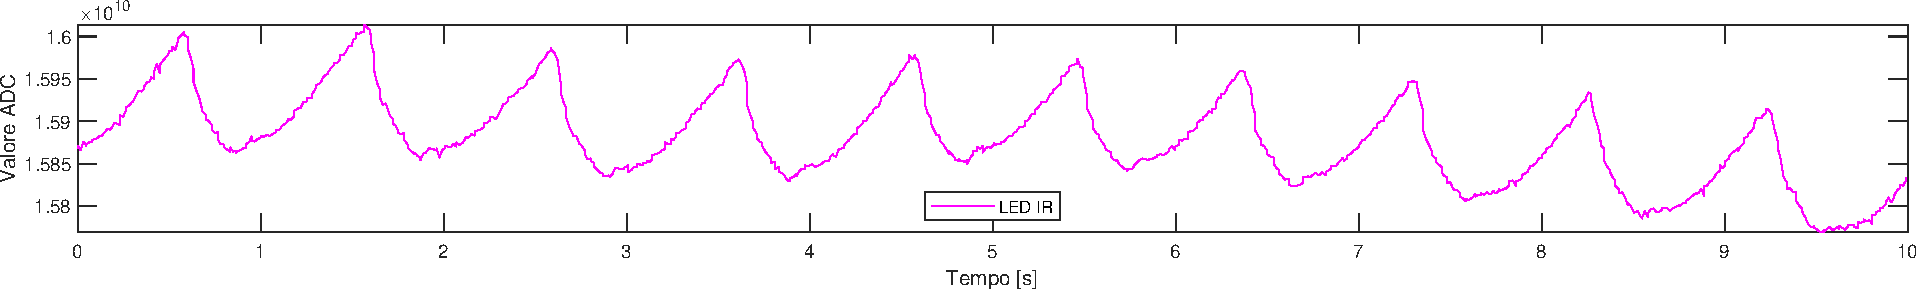
\includegraphics[width=1\linewidth]{ImageFiles/Misure Preliminari/Soggetto 2/max86916/fronte_ired}
	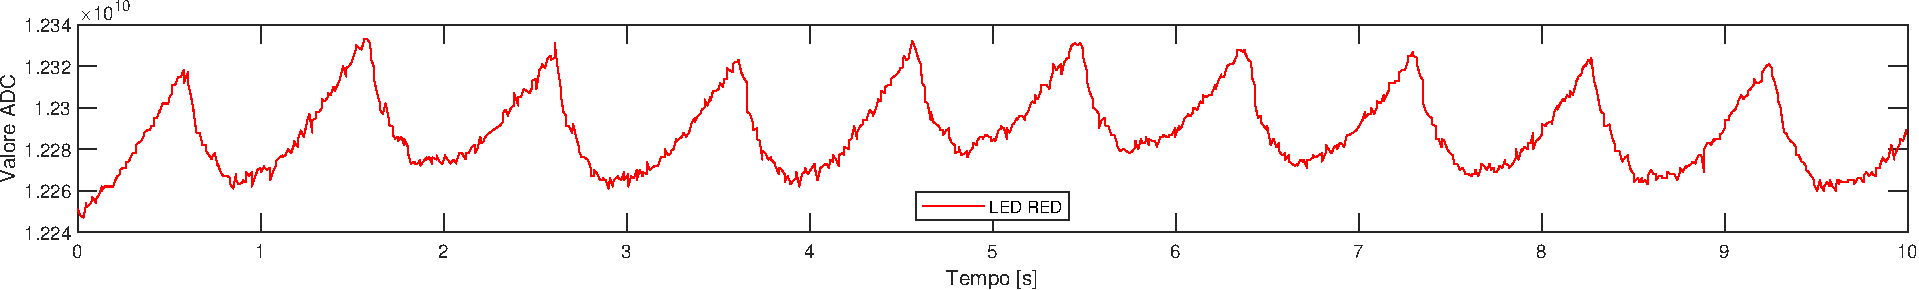
\includegraphics[width=1\linewidth]{ImageFiles/Misure Preliminari/Soggetto 2/max86916/fronte_red}
	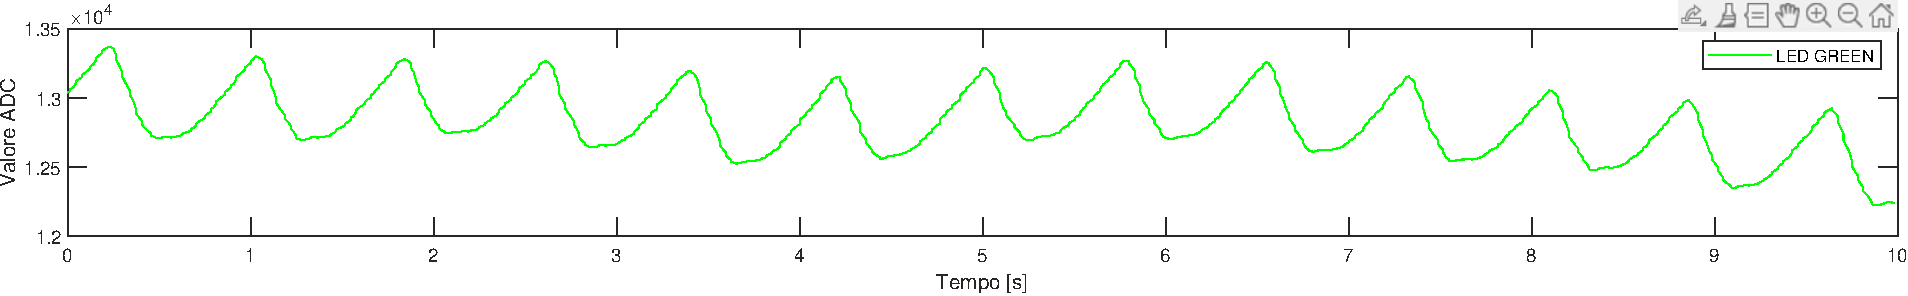
\includegraphics[width=1\linewidth]{ImageFiles/Misure Preliminari/Soggetto 2/max86916/fronte_green}
	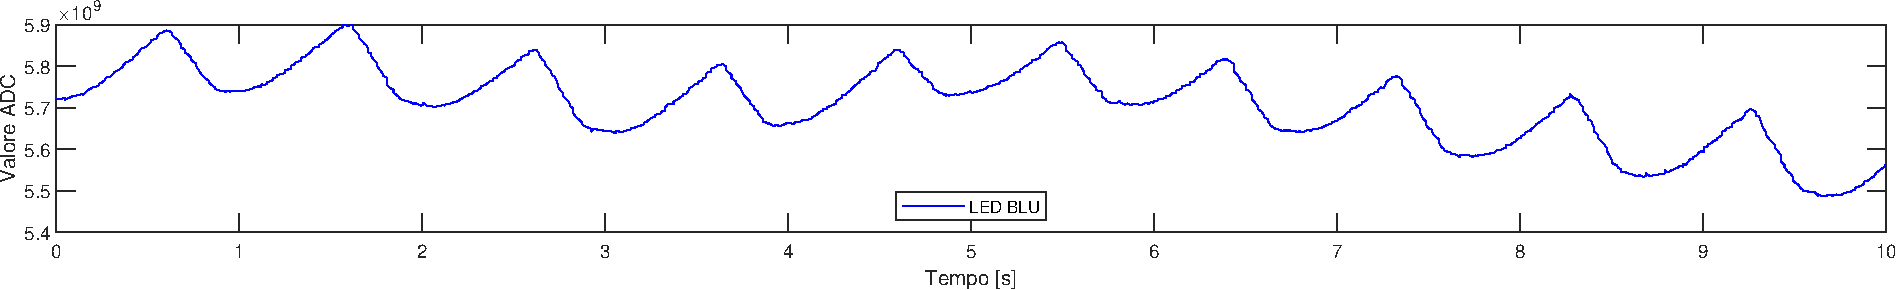
\includegraphics[width=1\linewidth]{ImageFiles/Misure Preliminari/Soggetto 2/max86916/fronte_blu}
	\caption{MAX86916: segnali PPG acquisiti sulla fronte.}
	\label{fig:soggetto2_MAX86916_fronte}
\end{figure}

\clearpage

Di seguito sono riportate le acquisizioni effettuate utilizzando il sensore \textbf{MAXM86161} su una finestra temporale di 10 secondi. Le acquisizioni ottenute sono state elaborate con un filtro a media mobile in modo da evidenziare il segnale fotopletismografico.

\subparagraph{Polpastrello indice sinistro}
Il segnale PPG ottenuto dall'acquisizione sul polpastrello del dito indice sinistro, e successivamente filtrato, risulta essere di buona qualità, con tutti i picchi caratteristici del segnale PPG. Infatti, come si può notare dalla figura \ref{fig:soggetto2_MAXM86161_polpastrello}, sono ben visibili i picchi sistolici e diastolici. Questo risultato era prevedibile dal momento che il polpastrello è noto essere un ottimo sito di misura per segnali fotopletismografici. Il filtro è quello a media mobile, con una finestra di 10 campioni per il LED verde e di 20 per il LED rosso e 25 per quello infrarosso. I picchi del segnale sono 13, quindi la frequenza cardiaca stimata è di 78 battiti al minuto.
\begin{figure}[h]
	\centering
	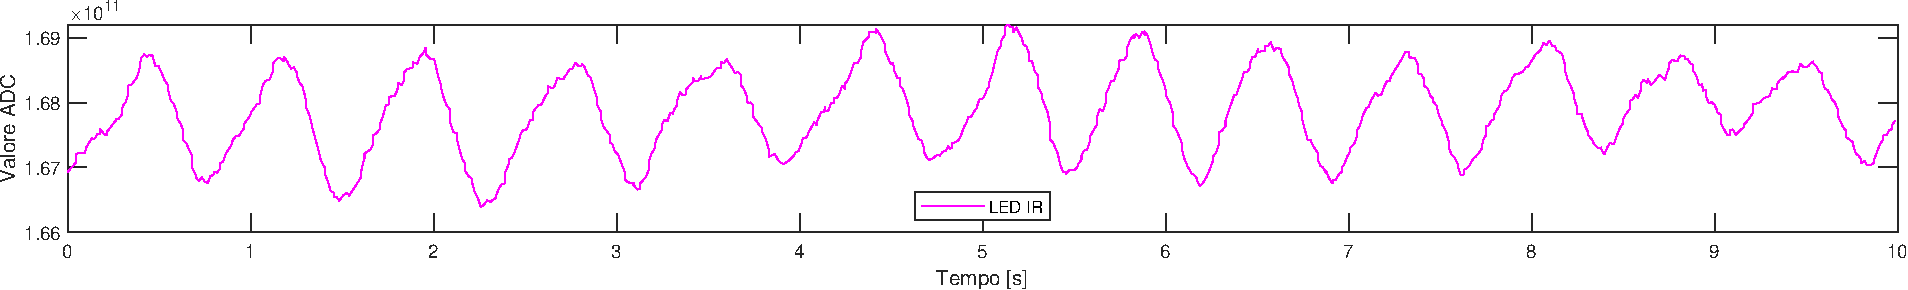
\includegraphics[width=1\linewidth]{ImageFiles/Misure Preliminari/Soggetto 2/maxm86161/polpastrello_ir_moving_avg}
	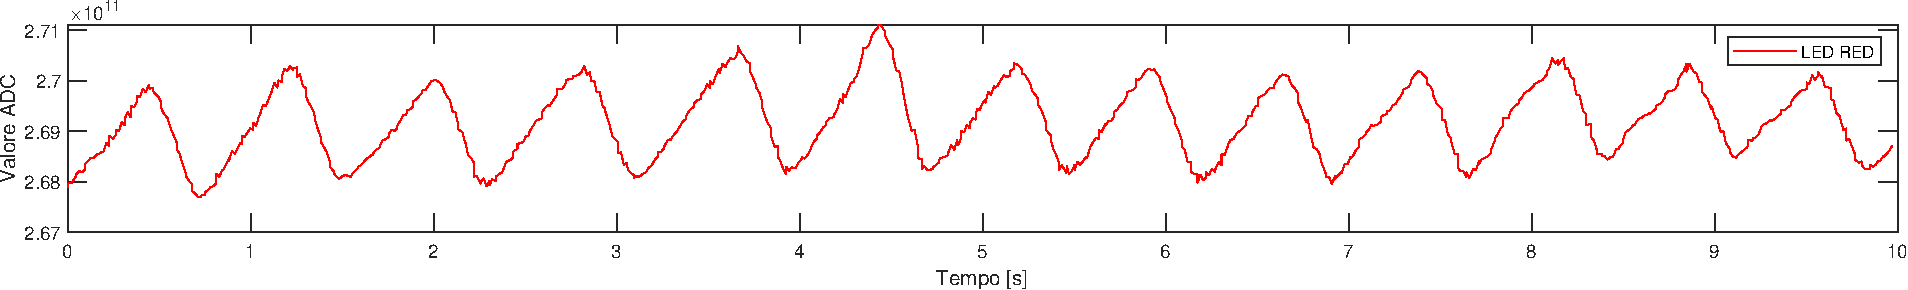
\includegraphics[width=1\linewidth]{ImageFiles/Misure Preliminari/Soggetto 2/maxm86161/polpastrello_red_moving_avg}
	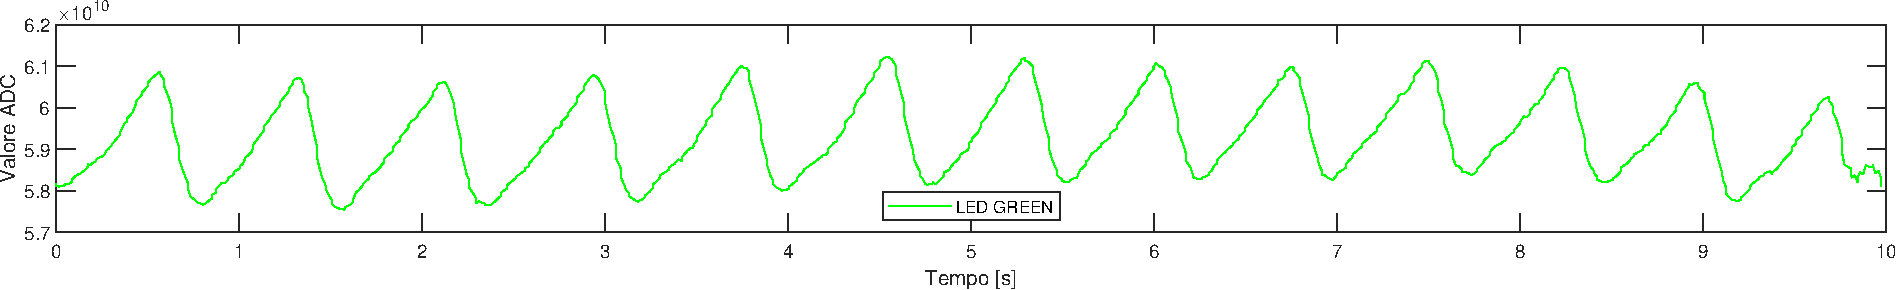
\includegraphics[width=1\linewidth]{ImageFiles/Misure Preliminari/Soggetto 2/maxm86161/polpastrello_green_moving_avg}
	\caption{MAXM86161: segnali PPG acquisiti sul polpastrello del dito indice sinistro.}
	\label{fig:soggetto2_MAXM86161_polpastrello}
\end{figure}
\clearpage
\paragraph{Lobo orecchio sinistro}
In figura \ref{fig:soggetto2_MAXM86161_lobo} sono riportati i risultati dell'acquisizione sul lobo dell'orecchio sinistro. Il segnale è stato filtrato con una finestra di 10 campioni per il LED verde, 30 per il LED rosso e 35 per quello infrarosso. La qualità dell'acquisizione è ancora molto buona, ma sempre leggermente inferiore a quella dell'acquisizione sul polpastrello, questo dovuto sempre alla difficoltà nella misura. Tuttavia, si possono apprezzare i picchi sistolici e diastolici, caratteristici del segnale PPG. I picchi contati sono 11, stimando una frequenza cardiaca di 66 battiti al minuto.
\begin{figure}[h]
	\centering
	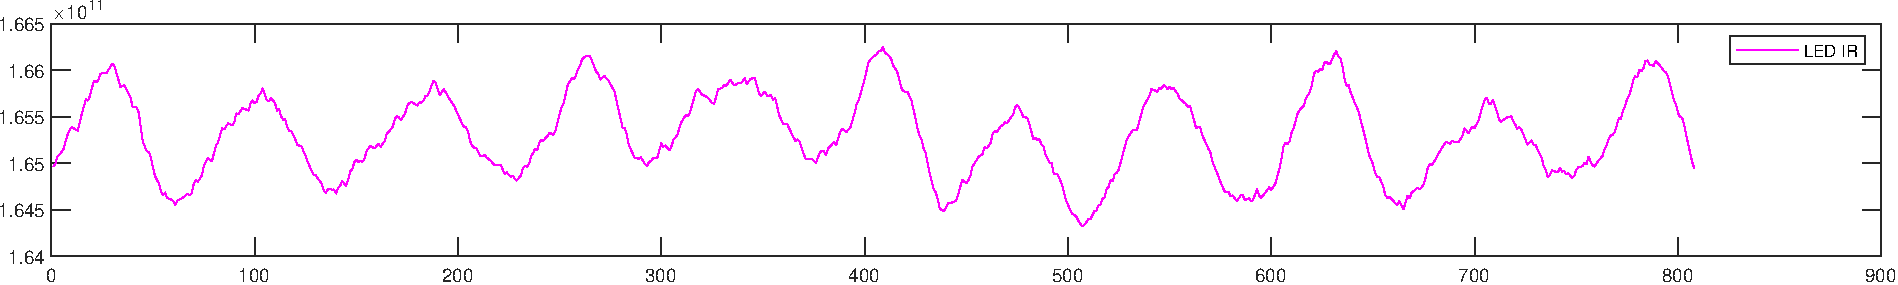
\includegraphics[width=1\linewidth]{ImageFiles/Misure Preliminari/Soggetto 2/maxm86161/lobo_ir_moving_avg}
	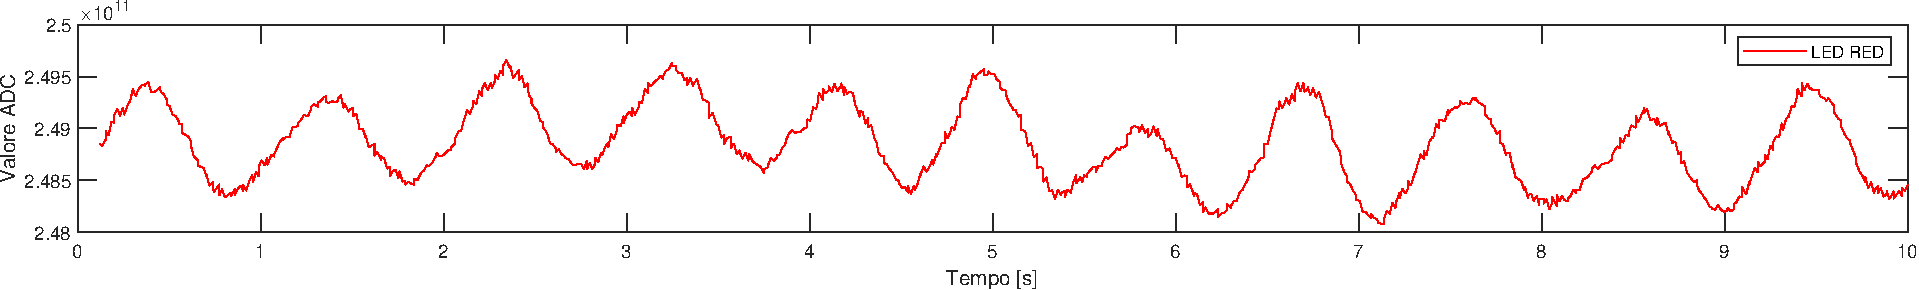
\includegraphics[width=1\linewidth]{ImageFiles/Misure Preliminari/Soggetto 2/maxm86161/lobo_red_moving_avg}
	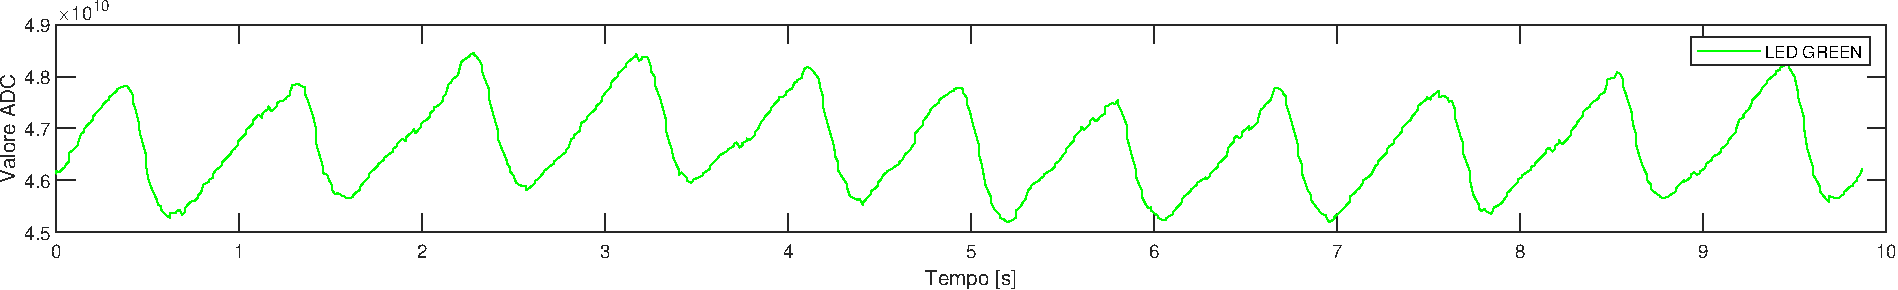
\includegraphics[width=1\linewidth]{ImageFiles/Misure Preliminari/Soggetto 2/maxm86161/lobo_green_moving_avg}
	\caption{MAXM86161: segnali PPG acquisiti sul lobo dell'orecchio destro.}
	\label{fig:soggetto2_MAXM86161_lobo}
\end{figure}

\clearpage

\subparagraph{Polso antero-interno sinistro}
L'acquisizione effettuata sul polso risulta invece molto rumorosa (Fig. \ref{fig:soggetto2_MAXM86161_polso}), specialmente per il segnale del LED infrarosso, mentre i segnali dei LED rosso e verde risultano avere una buona qualità. Nonostante ciò, sono ancora visibili i picchi caratteristici per tutti e tre i LED. Le finestre del filtro sono 15 campioni per il LED verde e 30 per i LED rosso e infrarosso. La frequenza cardiaca stimata è di 66 battiti al minuto.

\begin{figure}[h]
	\centering
	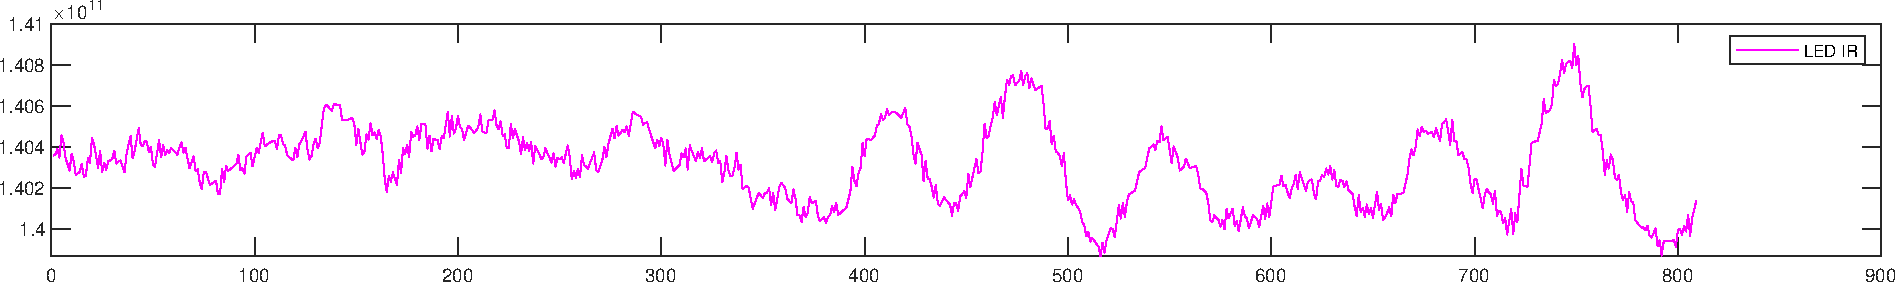
\includegraphics[width=1\linewidth]{ImageFiles/Misure Preliminari/Soggetto 2/maxm86161/polso_inferiore_ir_moving_avg}
	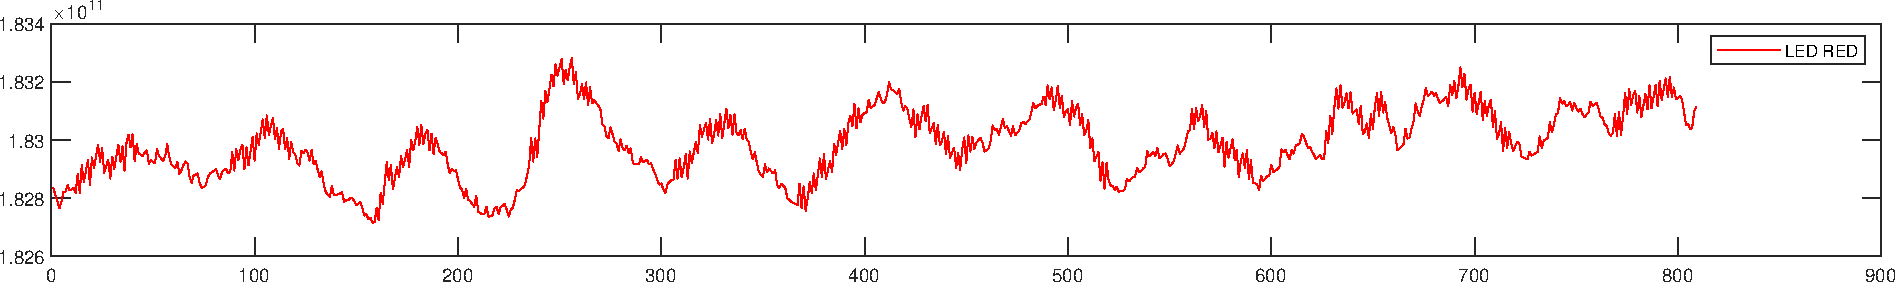
\includegraphics[width=1\linewidth]{ImageFiles/Misure Preliminari/Soggetto 2/maxm86161/polso_inferiore_red_moving_avg}
	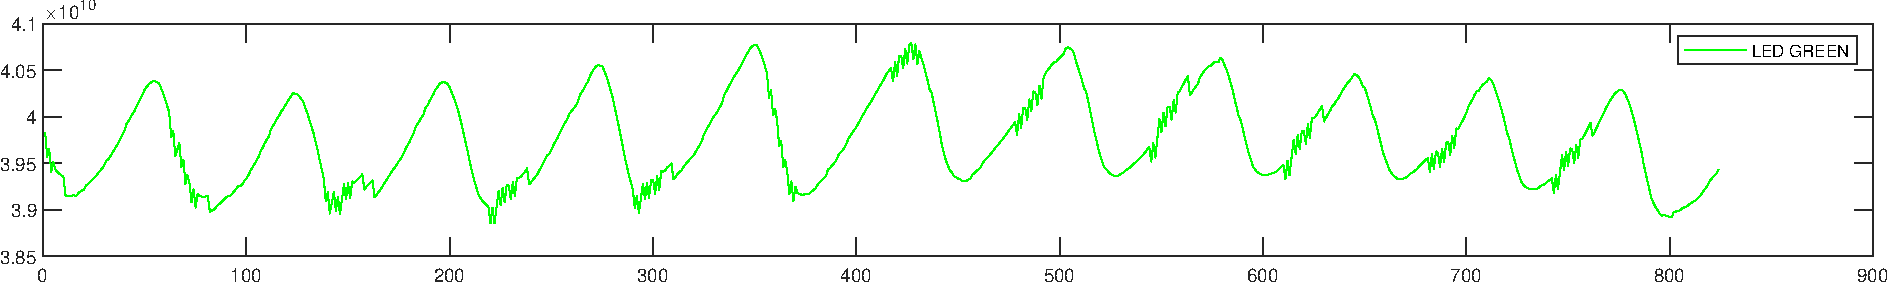
\includegraphics[width=1\linewidth]{ImageFiles/Misure Preliminari/Soggetto 2/maxm86161/polso_inferiore_green_moving_avg}
	\caption{MAXM86161: segnali PPG acquisiti sul polso destro.}
	\label{fig:soggetto2_MAXM86161_polso}
\end{figure}

\clearpage

\subparagraph{Fronte}
I segnali ottenuti dall'acquisizione sulla fronte, riportati in figura \ref{fig:soggetto2_MAXM86161_fronte}, sono molto buoni per il LED verde, mentre risultano affetti da rumore quelli dei LED rosso e infrarosso. Il filtro applicato ha una finestra di 10 campioni per il LED verde e 35 per i LED rosso e infrarosso. I picchi individuati sono 11, stimando una frequenza cardiaca di 66 battiti al minuto.

\begin{figure}[h]
	\centering
	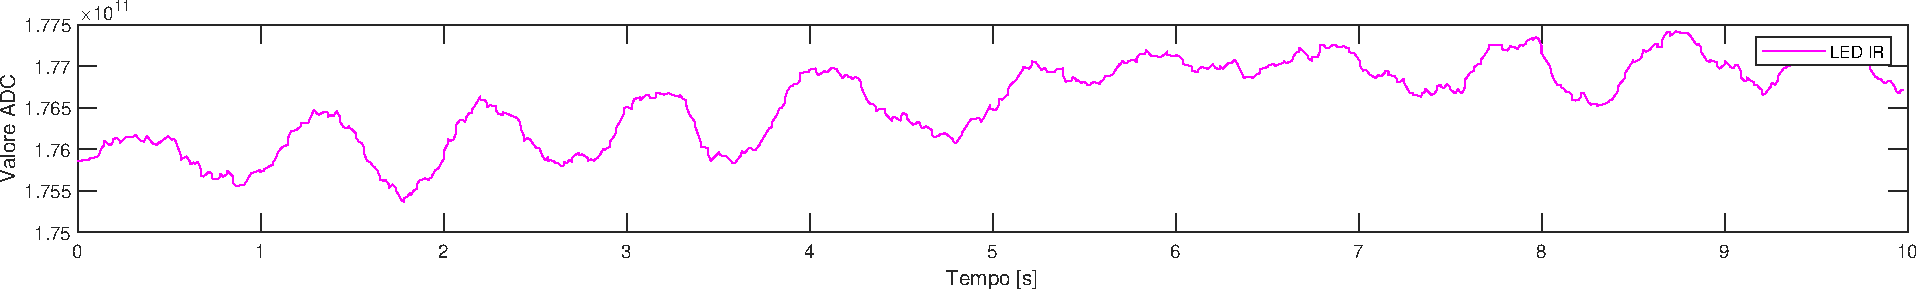
\includegraphics[width=1\linewidth]{ImageFiles/Misure Preliminari/Soggetto 2/maxm86161/fronte_ir_moving_avg}
	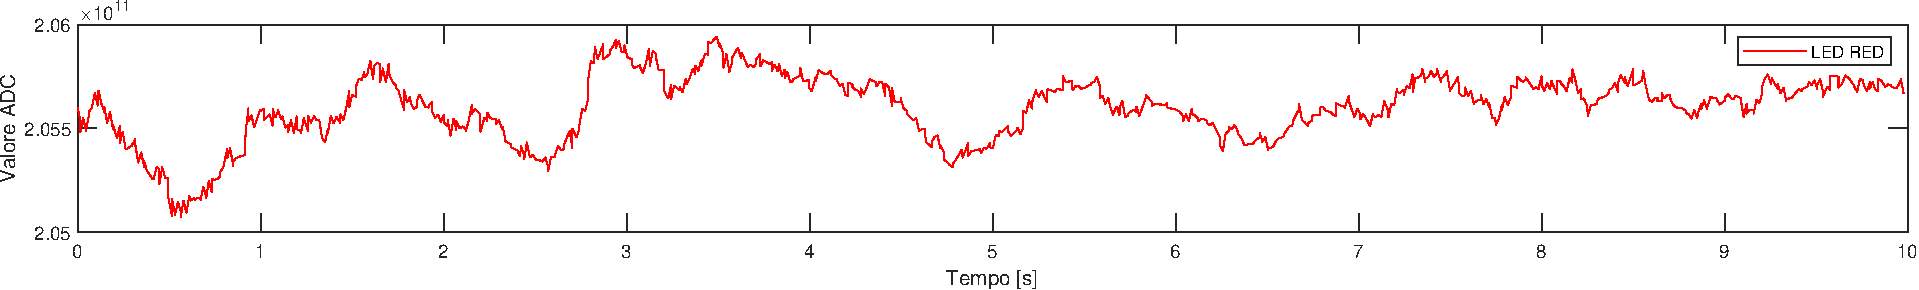
\includegraphics[width=1\linewidth]{ImageFiles/Misure Preliminari/Soggetto 2/maxm86161/fronte_red_moving_avg}
	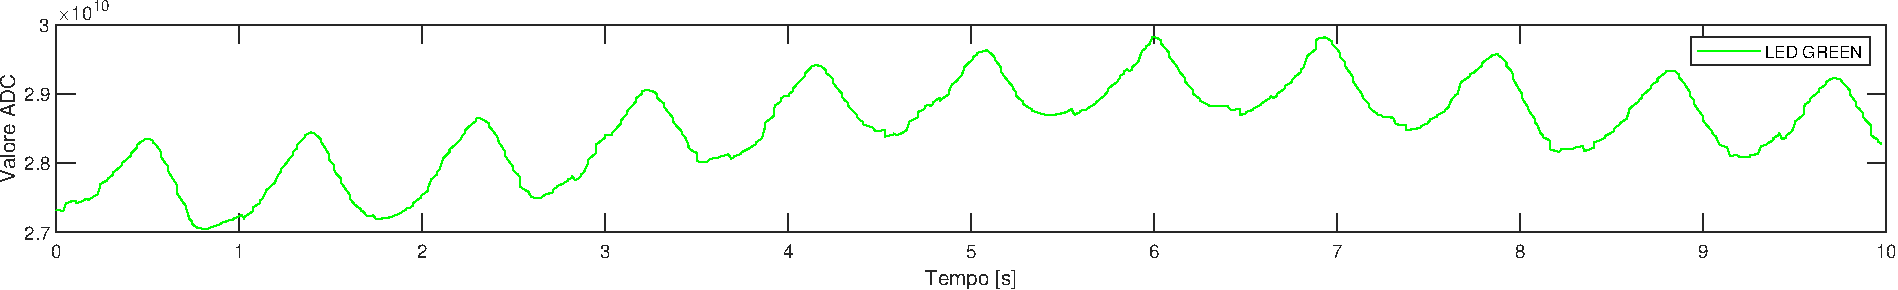
\includegraphics[width=1\linewidth]{ImageFiles/Misure Preliminari/Soggetto 2/maxm86161/fronte_green_moving_avg}
	\caption{MAXM86161: segnali PPG acquisiti sulla fronte.}
	\label{fig:soggetto2_MAXM86161_fronte}
\end{figure}


\clearpage